\documentclass[tikz, border=2mm]{standalone}
\usepackage{../tikz-preamble}

% arara: pdflatex: { draft: yes }
% arara: pdflatex: { synctex: no }
% arara: latexmk:  { clean: partial }
\begin{document}
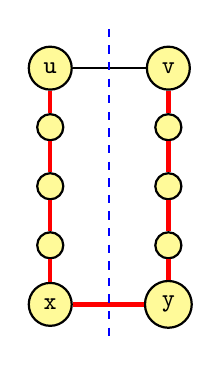
\begin{tikzpicture}[
	scale=1,
	transform shape,
	thick,
	font=\ttfamily\bfseries\small
]
\tikzset{
    mynode/.style = {circle, draw=black, align=center,fill=yellow!40},
    edgen/.style = {-},
    edger/.style = {-, ultra thick, red},
}
	\node[mynode] at (0.0,3.0) (u) {u};
	\node[mynode] at (0.0,2.25) (u1) {};
	\node[mynode] at (0.0,1.50) (u2) {};
	\node[mynode] at (0.0,0.75) (u3) {};
	\node[mynode] at (1.5,2.25) (v1) {};
	\node[mynode] at (1.5,1.50) (v2) {};
	\node[mynode] at (1.5,0.75) (v3) {};
	\node[mynode] at (1.5,3.0) (v) {v};
	\node[mynode] at (0.0,0.0) (x) {x};
	\node[mynode] at (1.5,0.0) (y) {y};

	\draw[edger] (x) to (y);
	\draw[edger] (u) to (u1);
	\draw[edger] (u1) to (u2);
	\draw[edger] (u2) to (u3);
	\draw[edger] (u3) to (x);
	\draw[edger] (v) to (v1);
	\draw[edger] (v1) to (v2);
	\draw[edger] (v2) to (v3);
	\draw[edger] (v3) to (y);
	\draw[edgen] (u) to (v);

	\path[draw,dashed,blue] (0.75,3.5) -- (0.75, -0.5);
\end{tikzpicture}
\end{document}